% Slide: End-to-End Impact on SLSQP (Corrected Layout)
\begin{frame}{Results: End-to-End Impact on SLSQP}

  \begin{columns}[c,onlytextwidth] % Vertically centered

    % ----- LEFT: The SLSQP performance graph -----
    \pause
    \column{0.6\textwidth}
    \begin{figure}
      \centering
      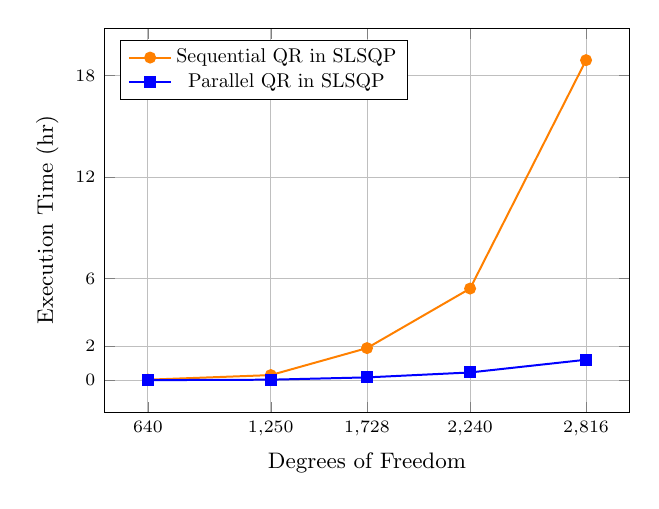
\begin{tikzpicture}[scale=0.9, transform shape]
        \begin{axis}[
            xlabel={Degrees of Freedom},
            ylabel={Execution Time (hr)},
            myAxisStyle/.style={
                tick label style={font=\scriptsize},
                label style={font=\small},
                grid=both,
                width=9cm,
                height=7cm
            },
            myAxisStyle,
            legend style={nodes={scale=0.8, transform shape}},
            xtick={640,1250,1728,2240,2816},
            ytick={0,2,6,12,18},
            legend pos=north west
            ]
            \addplot[orange, mark=*, thick] coordinates { (640,0.02908) (1250,0.3004) (1728,1.89514) (2240,5.415) (2816,18.91215) };
            \addlegendentry{Sequential QR in SLSQP};
            \addplot[blue, mark=square*, thick] coordinates { (640,0.001454) (1250,0.02879) (1728,0.16458) (2240,0.456) (2816,1.20716) };
            \addlegendentry{Parallel QR in SLSQP};
        \end{axis}
      \end{tikzpicture}
    \end{figure}

    % ----- RIGHT: Concise bullet points for context and results -----
    \column{0.4\textwidth}
    \begin{block}{Context}
      \begin{itemize}
        \item We integrated our parallel QR into the full SLSQP solver.
        \item \textbf{DOF (Degrees of Freedom):} Total problem variables. More DOF = larger matrix.
      \end{itemize}
    \end{block}
    
    \pause
    \begin{alertblock}{Final Result}
      At 2,816 DOF:
      \begin{itemize}
        \item Sequential: \textbf{18.9 hours}
        \item Parallel: \textbf{1.2 hours}
        \item \textbf{> 15x Speedup}
      \end{itemize}
    \end{alertblock}

  \end{columns}
\end{frame}